\chapter{Model Description}\label{cha:model_description}



%********************* NEW SECTION *********************
%-------------------------------------------------------
\section{Morphology} \label{sec:morphology}
The airway morphology is represented by a generic network of straight branching ducts, which terminate in trumpet-like compartments.
In that sense, straight ducts are used to represent the bigger, non-compliant airways, where convective transport is dominant.
The dimensions of the trachea and the two main bronchi are defined by anatomical data described by \citet{Weibel1963}.
In addition, the functional residual capacity (FRC) that is, the air volume that remains in the lung after a tidal expiration, serves as scaling factor for the trachea and therefore accounts for teh scaling of the entire airway network.
The length of the scaled trachea is defined as
\begin{equation}
l_0 = {l_0}_\mathrm{W}\left(\frac{\mathrm{FRC}}{\mathrm{FRC}_\mathrm{W}}\right)^{1/3} \cc
\end{equation}
Where the subscript $W$ indicates a reference quantity from the data by \citet{Weibel1963}.
For airways past the main bronchi, the scheme for a regular branching asymmetry introduced by \cite{Majumdar2005} was applied.
In this scheme, each duct-like airway bifurcates in a major and a minor daughter.
In the airway network every parent, minor and major daughter share a common node.
The dimensions of the daughter airways, namely their diameter and length, are different fractions of the dimension of their common parent duct,
\begin{equation} \label{eqn:bifurcationRule}
\begin{split}
{d_{z+1}}_{\mathrm{maj}} &= d_{z}\kappa_\mathrm{maj} \quad\text{with}\quad \kappa_\mathrm{maj} = (1-r)^{1/\eta}\\
{d_{z+1}}_{\mathrm{min}} &= d_{z}\kappa_\mathrm{min} \quad\text{with}\quad \kappa_\mathrm{min} = r^{1/\eta} \pp
\end{split}
\end{equation}
Here, $d_z$ is the diameter of a duct at generation $z$, and $r$ and $\eta$ denote the asymmetry parameter and reduction rate, respectively.
The same scheme was used to define the length of airways.
In their study, \citet{Majumdar2005} presented values $r = 0.326$ and $\eta = 2.97$ for which the resulting structure best represents the human lung on a statistical basis.
In the present model this bifurcation scheme is applied until the diameter of a duct is smaller than a limit diameter $d_\mathrm{lim} = 1.8 \unit{mm}$, typically chosen to represent bronchi at the 8th-12th generation.
The last generation of duct-like airways depends on the limit diameter and may vary within the model, due to the asymmetric bifurcation scheme.
The unit distal to an ending duct constitutes a lobule and is modelled using a trumpet-like compartment (trumpet lobule).
The lobule as defined here contains, apart from the acini and the respiratory bronchioles, the last generations of conductive airways.
Compared to the duct-like, rigid airway, the trumpet lobule can be interpreted as a compartment with diverging, time-variable cross-section (see Figure \ref{fig:trumpetSketch}).
The number of these trumpet lobules is equal to the number of terminal ducts, which again is determined by the limit diameter and the FRC.
In general, each trumpet can have distinct geometrical and mechanical properties.
An important constraint, however, is that the total volume of the model (duct-like airways and trumpet lobules) under static conditions equals a predefined FRC.
In order to simulate the effects of lung structural inhomogeneity on the MBW test, properties of both the stiff and the compliant parts of the model can be modified (see Section \ref{sec:model_modifications} for more informations on possible model modifications).
Figure illustrates a sketch of a model lung showing the relative scales of a network of airways defined by the bifurcation rule (Equation (\ref{eqn:bifurcationRule})).
A detailed mathematical description of the trumpet, its geometrical and dynamical properties, can be found in Section \ref{ssec:lobules}.

\begin{figure}[tb]
\centering
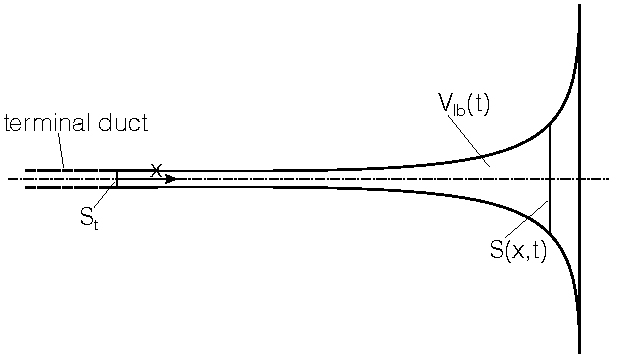
\includegraphics[width=0.5\textwidth]{figures/trumpetmodel}
\caption{Schematic representation of a trumpet-lobule with inlet cross-section $S_\ter$, dynamic cross-section $S_\lb(x,t)$ and volume $V_\lb(t)$}
\label{fig:trumpetSketch}
\end{figure}


%********************* NEW SECTION *********************
%-------------------------------------------------------
\section{Mathematical models} \label{sec:mathematial_model}


%****************** new sub-section ********************
\subsection{Ventilation} \label{ssec:ducts}
Lung ventilation is simulated by means of a lumped parameter (0-dimensional) model illustrated in Figure \ref{fig:lumpedparametermodel}.
For the duct-like airways purely resistive elements were used.
During normal breathing, airflow in the lung is unsteady and inertia plays a considerable role regarding the flow resistance in bigger airways until the tenth generation \citep{Kaczka2011}.
The theory by \citet{Womersley1957} for pulsatile flow in tubes was therefore applied.
In general, the pressure difference between two subsequent nodes with node index $i$ and $j$ in the network reads.
Here $Q_{ij}$ is the flow rate in direction of the negative pressure gradient, and the hydrodynamic resistance $R_{ij}$ depends on the radius $r_{ij}$ and the length $l_{ij}$ of the conducting airway between two nodes, and on the breath period $\mathrm{TB}$.

\begin{figure}[tb]
\centering
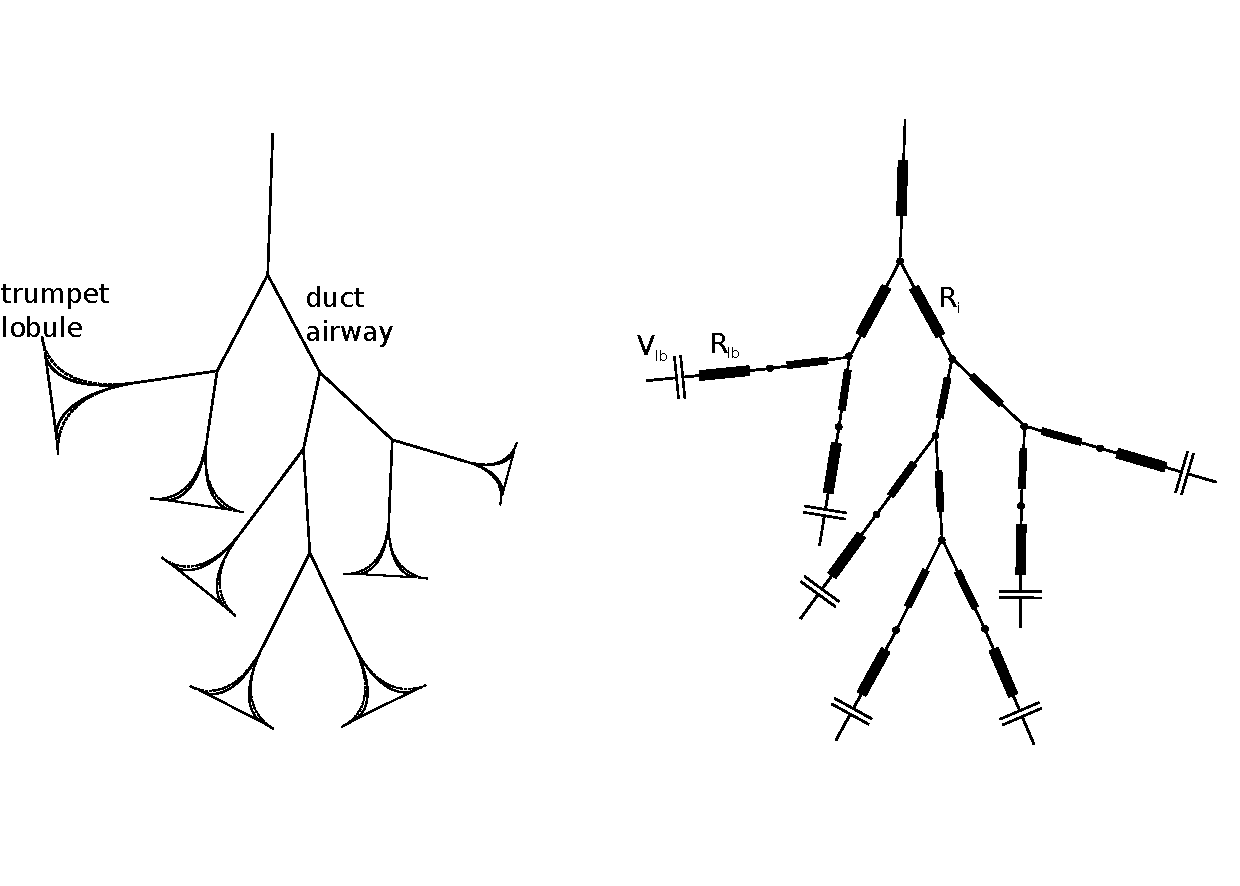
\includegraphics[width=0.5\textwidth]{figures/lumpedparametermodel}
\caption{Left, Network of duct and trumpet-like elements used for the upper and lower airways, respectively. Right, corresponding lumped parameter model composed of resistances and compliances.}
\label{fig:lumpedparametermodel}
\end{figure}


\subsubsection{Pressure volume relation in trumpet lobules}
The trumpet model, which mainly represents compliant, peripheral airways (lobules) is composed of a nonlinear compliance (elastic pressure, $p_\mathrm{el}$) element and a resistance (pressure loss, $p_\mathrm{diss}$) element, acting in series between a node with index $i$, corresponding to a terminal duct, and the pleural gap.
The corresponding pressure difference is defined as
\begin{equation} \label{eqn:constitutiveLaw}
p_i - p_\mathrm{pl} = \underbrace{\beta\e^{\gamma V_\mathrm{lb}^0}\left(\e^{\gamma \tilde{V}_\mathrm{lb}} - 1\right)}_{\text{\footnotesize{elastic pressure, }} p_\mathrm{el}} + \underbrace{R_\mathrm{lb}Q_\mathrm{lb}}_\text{\footnotesize{dissipation}}\cc
\end{equation}
where $R_\lb$, $V_\lb(t) = V_\lb^0 + \tilde{V}_\lb$ and $Q_\lb$ denote the flow resistance and the volume of, respectively the flow rate into, a trumpet lobule past a terminal duct-like airway, $V_\lb^0$ is the lobule volume at FRC and $\tilde{V}_\lb$ is the dynamic volume during breathing.
The shape parameters $\beta$ and $\gamma$ are used to define and modify the compliance of the trumpet lobule.
More information on the mechanical properties of the model can be found in the Section \ref{sec:model_modifications}.

Mass conservation has to be satisfied in the network.
Thus, in each node, the flow rates had to be balanced $\sum Q = 0$, and for the lobule model the flow rate of the terminal duct $Q_\ter$ equals the change of volume of the lobule, thus
\begin{equation}
  Q_\ter = \frac{\mathrm{d} V_\lb}{\mathrm{d} t}
\end{equation}
From these relations, a system of differential algebraic equations (DAE) results.
Together with appropriate boundary conditions, the DAE system governs the flow distribution in the lumped parameter model.

From a physiological point of view, during inspiration, airflow from the mouth and the nose moves to the alveolar membrane as a result of the motion of the diaphragm and the thoracic cavity, causing a volume increase and a pressure decrease in the pleural cap.
This negative (relative) pressure in the pleural gap causes a pressure gradient across the peripheral lung tissue and along the airways to the mouth and nose.
In that sense, obvious boundary conditions for the lumped parameter model (LPM) would be the pleural pressure and the pressure at the mouth. However, pleural pressure data is in general not obtained during clinical routine and therefore not accessible.
Instead, flow rate data at the mouth can be easily measured by flowmeters (e.g. in the multiple breath washout test).
Imposing boundary conditions for pressure and flow at the mouth allows solving the DAE with unknown pleural pressure.
To this end, a spatially uniform pleural pressure is assumed, which varies over time according to the prescribed volume change and the material law of the lung tissue.
A detailed description of the numerical implementation of the lumped parameter model is provided in Section \ref{ssec:ventilation}.


%****************** new sub-section ********************
\subsubsection{Trumpet lobule geometry} \label{ssec:trumpet_lobule_geometry}
For the trumpet model representing the lobules and their peripheral airways, a model for the total cross-section of the trumpet lobule $S_\lb = S_\lb(x,t)$, as well as for the mean advection velocity $u_\lb(x,t)$ had to be derived.
From the LPM the flow rate at the inlet of each trumpet $Q_\ter(t)$ and the total volume of the trumpet $V_\lb(t) = \int_0^t Q_\ter\d t + {V_\lb}^0$ was known.
The initial volume of the trumpet lobule, $V_\lb(t=0) = {V_\lb}^0$, followed from FRC-based scaling of the lung model.
Assuming a uniform homothety ratio of $\kappa = 0.85$ \cite{Weibel1963} for airways lumped in a trumpet lobule, the total change of cross-section along the streamwise coordinate $x$ can be described as

\begin{equation}\label{eqn:crosssection}
S(x,0) = S_\ter\hat{\kappa}^{z(x)}\cc \quad\text{with}\quad \hat{\kappa} = 2\kappa^2
\end{equation}
where $S_\ter$ is the cross-section of the terminal duct and $z(x)$ is the generation at absolute position $x$ with respect to the inlet of the trumpet lobule, both with respect to the terminal duct where $z = x = 0$.
Considering $l_\ter$ to be the length of the terminal duct, the cumulative length at generation $z$ (with respect to the inlet of the lobule) would be $\sum_{k=1}^z l_\ter\kappa^k$.
The limes of this sum for $z\rightarrow\infty$ is

\begin{equation}
\lim_{z \to \infty}\sum_{k=1}^z l_\ter\kappa^k = l_\ter\kappa/(\kappa - 1)) =: L \pp
\end{equation}

From these relations, an expression for the the generation in function of the distance to the inlet of the trumpet can be computed,

\begin{equation}\label{eqn:zofx}
z(x) = \frac{\log{\left[x\;\frac{\kappa - 1}{\kappa\;l_\ter} + 1\right]}}{\log{(\kappa)}}\pp
\end{equation}

Using equation (\ref{eqn:crosssection}) together with (\ref{eqn:zofx}) for further treatment of the lobule model becomes a rather cumbersome task.
We therefore sought a model $S_\lb(x,t)$, which approximates Equation (\ref{eqn:crosssection}) but allows to derive an analytical expression for $u_\lb(x,t)$.
To this end, we used a power law of the form

\begin{equation}\label{eqn:crosssectionModel}
S_\lb(x,t) = p_1 x^{n_1} + p_2 x^{n_2} + S_\ter\cc
\end{equation}

with $n_1, n_2 = 16, 2$, where the coefficients $p_1$ and $p_2$ were defined such that the $S_\lb$ intersects with Equation (\ref{eqn:crosssection}) at a chosen generation $z^\star$, and the prescribed initial volume $V_\lb^0$ of the trumpet lobule is obtained for a given length $l_\lb$ of the trumpet lobule.
The coefficients were thus defined by the following linear system

\begin{figure}[tb!]
  \centering
  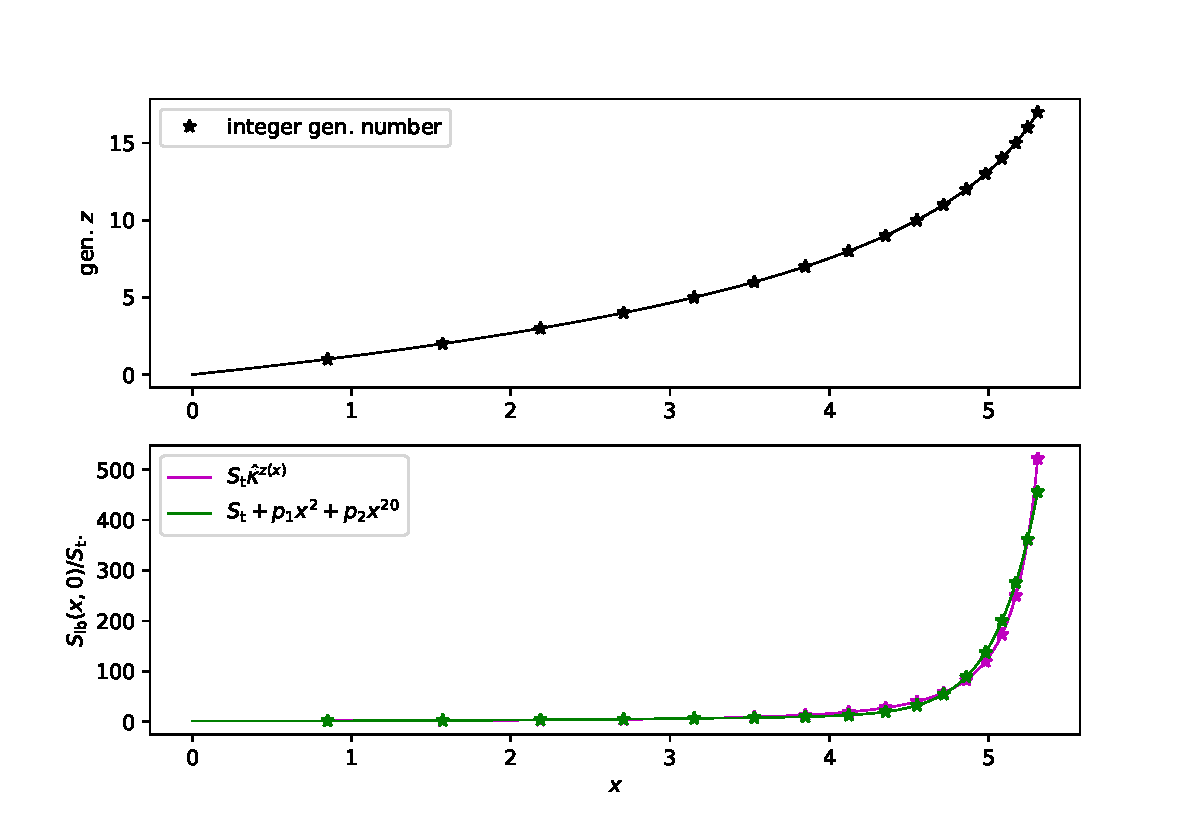
\includegraphics[width=1.0\textwidth]{figures/trumpet_geometry}
  \caption{Above: the generation $z$ plotted as function of the cumulative length or distance $x$ with $l_\ter = d_\ter = unity$. The solid line indicates the function described by equation (\ref{eqn:zofx}). Below: The cross-section as it follows from equation (\ref{eqn:crosssection}) (magenta) and the model (\ref{eqn:crosssectionModel}) (green) where $p_1$ and $p_2$ were defined to yield the same integral as the exponential law and intersects at generation $z^\star = 5$ ($z = 0$ at trumpet inlet).}
  \label{fig:trumpet_geometry}
\end{figure}

\begin{equation} \label{eqn:linearSystemCoeff}
\left[\begin{array}{c c} {x^\star}^{n_1}              & {x^\star}^{n_2} \\
                         \frac{l_\lb^{n_1+1}}{n_1 + 1} & \frac{l_\lb^{n_1+1}}{n_1 + 1} \\
      \end{array}\right]
\left(\begin{array}{c} p_1 \\
                       p_2 \\
      \end{array}\right)
=
\left(\begin{array}{c} S^\star - S_\ter \\
                       V_\mathrm{lb}^0 - S_\ter\;l_\lb\\
      \end{array}\right)
\end{equation}

with $S^\star = S_\lb(x^\star, 0)$ and $z^\star = z(x^\star)$.

In Figure \ref{fig:trumpet_geometry}, a comparison between equations (\ref{eqn:crosssection}) and (\ref{eqn:crosssectionModel}) shows a good agreement.
The actual length of the trumpet model was defined based on the cumulative length

\begin{equation}
l_\lb = \sum_{k=1}^{z_\mathrm{max}} l_\ter\kappa^k
\end{equation}

where $l_\lb = \approx0.98 L$ follows for a lobule with $z_\mathrm{max} = 16-18$ generation.
The system (\ref{eqn:linearSystemCoeff}) determined the initial (or end-expiratory) trumpet shape $S_\lb(x,0)$.
During breathing the cross-section widens.
Therefore the first coefficient of the power law was set to be a time-depending parameter $p_1 = p_1(t)$.
After the initial shape of the trumpet lobule was defined (using Equations (\ref{eqn:linearSystemCoeff})), $p_1(t)$ was updated according to the lobular volume $V_\lb(t)$
\begin{align}
  V_\lb(t) &= \int_0^{l_\lb} S_\lb(x,t)\;\d x \\
  \Rightarrow p_1(t) &= \frac{n_1+1}{l_\lb^{n_1+1}} \left[ V_\lb(t) - \frac{l_\lb^{n_2+1}}{n_2 + 1} p_2 - S_\ter l_\lb\right] \label{eqn:shapeParameter}
\end{align}

This determined the shape of the trumpet acinus at any time.
An important feature of the model (\ref{eqn:crosssectionModel}) is the major contribution of peripheral airway (where $x$ is close to $l_\lb$) to the overall expansion of the lung.


%****************** new sub-section ********************
\subsection{Gas transport} \label{ssec:lobules}
To model the time-variable distribution of tracer gases in the lung, typically nitrogen ($N_2$) or sulfur-hexafluoride ($SF_6$), a one-dimensional transport equation for a scalar variable representing the concentration $c = c(x,t)\in[0,1]$ (normalised with the maximum value), is solved with a finite difference method (see Section \ref{ssec:gas}).
Simulation of MBW involves the computation of gas concentration in all model airways over multiple breath periods.
Moreover, only inert gases were considered.
For this case, the dominant transport mechanisms are advection by the carrier gas (ambient air) and diffusion.
The molecular mass of $N_2$ as the tracer gas is much smaller than that of the carrier gas.
Therefore, the assumption of a diluted gas is made, where molecular diffusion of a tracer gas in a carrier gas depends only on the physical properties of the two gases involved \cite{Cussler2009}.
As a further assumption, these properties (temperature, molecular velocity, etc.) and therefore the diffusivity of a tracer gas are considered to be constant in the lung and throughout the breath cycle.
The coordinate (here denoted with $x$), along which the transport process takes place, is the center line of a model airway, hence along each duct-like airway and along each lobule trumpet.
The 1D approximation entails consideration of averaged (lumped) quantities within a cross-section, or in case of the trumpet model, within the total cross-section of all airways at a given position $x$.
Advection-diffusion processes, taking place in a pipe-like geometry are subject to high radial velocity gradients.
As a consequence, high-concentration gas is transported (advected) along low-concentration gas increasing the interface of high concentration gradients and therefore increasing the average diffusivity within a cross-section.
In the human lung this phenomena can take place on different scales: In the upper airway, where the Reynolds number $\Rey = u d \rho/\mu$ is in the order of $10'000$, turbulent flow strongly enhances mixing.
In smaller airways ($\Rey < 2'000$), Poiseuille flow with a parabolic velocity profile can be assumed.
Enhanced diffusion due to high velocity gradients is usually modelled based on the concept of Taylor dispersion, where the local diffusion coefficient is a function of the local Peclet number \citet{Cussler2009},
\begin{equation}
\hat{D} = D\left(1 + \frac{1}{192}\Pe^2\right) \pp
\end{equation}
Here, $\hat{D}$ and $D$ are the effective and molecular diffusion coefficient, respectively, and $\Pe$ is the Peclet number defined with the (local) mean velocity $u$ and the (local) airway diameter $d$.

In the lung model, the gas concentration evolves in a network of one-dimensional domains.
To this end, the transport equation is solved in each of these sub-domains separately (domain decomposition approach), applying a coupling of concentration values from different domains in bifurcation nodes.
A transport equation of the following general form is considered
\begin{equation} \label{eqn:transportEquation}
\frac{\partial (Sc)}{\partial t} + \frac{\partial F}{\partial x} = 0\cc \quad\text{with the flux}\quad F = S_\mathrm{ad} u c - S\hat{D}\frac{\partial c}{\partial x} \pp
\end{equation}
Here, we distinguished between the total cross-section $S(x,t)$ and the cross-section $S_\mathrm{ad}$ where advection with the carrier gas velocity $u(x,t)$ takes place.
At bifurcations the concentration flux has to be conserved $\sum F = 0$.
The geometry of the trumpet lobule $S_\lb(x,t)$ (derived in Section \ref{ssec:trumpet_lobule_geometry}) allows a more specific form of Equation (\ref{eqn:transportEquation}) to be stated for the gas transport within trumpet lobules with non-constant cross-section (see \label{ssec:modified_advection_diffusion_equation}).



\subsubsection{Modified advection-diffusion equation} \label{ssec:modified_advection_diffusion_equation}
The derivation of the transport equation (Equation \ref{eqn:transportEquation}) is different for duct-like and trumpet-like airways in the lung model.
In the first case, the advection velocity directly results from the solution of the lumped parameter model (LPM, solving for node pressures $p_i$ and $p_j$, and the flow rate $Q_{ij}$ between the nodes $i$ and $j$) and is constant within a duct, $u_{ij} = Q_{ij}/{S_\mathrm{ad}}_{ij}$.
Furthermore, ducts are stiff and hence $S = S_\mathrm{ad} = \text{const}$.
Omitting the subscripts referring to nodes for briefity, the transport equation for a species concentration $c = c(x,t)$ in a duct-like airway can be written as an advection-diffusion-equation
\begin{equation} \label{eqn:advectionDiffusionDuct}
\frac{\partial c}{\partial t} + u\frac{\partial c}{\partial x} - \hat{D}\frac{\partial^2 c}{\partial x^2} = 0 \pp
\end{equation}


For a trumpet lobule with cross-section $S_\lb(x,t)$, an expression for the advection velocity in the trumpet model can be found introducing the 1D continuity equation for a non-constant cross-section,

\begin{equation} \label{eqn:continuityEquation}
\frac{\partial S_\lb}{\partial t} + \frac{\partial Q_\lb}{\partial x} = 0 \pp
\end{equation}

Using the model $S_\lb(x,t)$ introduced above, the first term becomes

\begin{equation}
  \frac{\partial S_\lb}{\partial t} = x^{n_1}\frac{\partial p_1}{\partial t} = x^{n_1}\frac{\partial p_1}{\partial V_\lb}\frac{\partial V_\lb}{\partial t} = x^{n_1} \frac{n_1+1}{l_\lb^{n_1+1}}\;Q_\ter
\end{equation}

Integrating the continuity equation then yields an equation for the flow rate

\begin{equation} \label{eqn:flowRateTrumpet}
\begin{split}
Q_\lb(x,t) &= -\int \frac{\partial S_\lb}{\partial t} \d x \\
       &= Q_\ter(t)\left[1 - \frac{x^{n_1+1}}{l_\lb^{n_1+1}}\right]
\end{split}
\end{equation}

The term in brackets is $1$ for $x=0$ and $0$ for $x = l_\lb$, which is in agreement with the condition of zero outflow at the end of the trumpet and follows from the constraint $Q_\ter = \d V_\lb / \d t$.
The advection velocity in the trumpet is related to the flow rate, $u_\lb(x,t) = Q_\lb(x,t)/S_\mathrm{ad}$, where for the advection cross-section the same model as for $S_\lb$ is used but half the initial lobular initial volume is used for the determination of the coefficients $p_1$ and $p_2$.

The transport equation (Equ. 6 and 7 in the main article) together with the continuity equation (\ref{eqn:continuityEquation}) can be rearranged for non constant $S_\lb(x,t)$ and $u_\lb(x,t)$ yielding an advection-diffusion equation with modified advection velocity

\begin{equation} \label{eqn:advectionDiffusionTrumpet}
\frac{\partial c}{\partial t} + \underbrace{\left[\frac{S_\mathrm{ad}}{S_\lb}u_\lb - \frac{\hat{D}}{S_\lb}\frac{\partial S_\lb}{\partial x} \right]}_{=\hat{u}}\frac{\partial c}{\partial x} - \hat{D}\frac{\partial^2 c}{\partial x^2} = 0
\end{equation}

In summary, equations (\ref{eqn:advectionDiffusionDuct}) and (\ref{eqn:advectionDiffusionTrumpet}) describe the gas transport in duct,
respectively trumpet-type airway models and equations (\ref{eqn:crosssectionModel}) and (\ref{eqn:flowRateTrumpet}) together with (\ref{eqn:shapeParameter}) describe the dynamics of the trumpet model.
The system is coupled with the ventilation LPM through the average flow velocity in each duct and into each trumpet.
The numerical solution method for the LPM and for the advection-diffusion equation are presented in S2\_Appendix and S3\_Appendix, respectively.



%********************* NEW SECTION *********************
%-------------------------------------------------------
\section{Model modifications} \label{sec:model_modifications}
An important application of the lung model is to simulate the effects of different functional and structural inhomogeneities within the lung.
I.e. non-uniform tissue compliance, non-uniform size of airway units (e.g. lobules, acini), and non-uniform flow resistance in small airways, affecting different parts of the lung.

\paragraph{Lobule Compliance: }
Tissue compliance can be tuned with the modification parameter $\phi$, which is used to define the shape parameter $\beta$ and $\gamma$ in Equation (\ref{eqn:constitutiveLaw}).
To this end we considered a mean lobular tidal volume $V_\lb^{TV} = TV/N_\lb$, where $TV$ is the tidal volume, and $N_\lb$ is the total number of trumpet-lobules.
The elastic component of the lobule mechanics can be called stiff if its maximum dynamic volume is smaller than $V_\lb^{TV}$, and soft otherwise.
The elastic pressure curve for lobules with distinct compliance is shown in Figure \ref{fig:lobuleMechanics}, where the shape parameter $\beta$ was defined as
\begin{equation} \label{eqn:compliance_modification}
\beta = \frac{p_\mathrm{lb}^{TV}}{\e^{\gamma V_\mathrm{lb}^0}(\e^{\gamma \phi V_\mathrm{lb}^{TV}} - 1)} \cc
\end{equation}
For instance, $\phi = 0.5, 1.0, 1.5$ can be used for a stiff, normal and compliant trumpet-lobule, respectively.
In the scaling of $\beta$ (Equation (\ref{eqn:compliance_modification})), a reference pressure amplitude $p_\lb^{TV} = 1500 \unit{Pa}$ can be assumed, which corresponds to a typical pressure range introduced by the pleural pressure.
The remaining shape parameter $\gamma$ accounts for the non-linearity of the elastic pressure law and is defined based on a point in the volume-pressure plane $(V_\lb^0 + 3/4\phi V_\lb^{TV}, 1/4 p_\lb^{TV})$, which has to be satisfied by equation (Equation (\ref{eqn:constitutiveLaw})).

\paragraph{Lobule Volume: }
The modification parameter $\theta$ is used to modify the residual volume of a trumpet lobule as ${V_\lb^0}_\mathrm{mod} = \theta V_\lb^{0}$.

\paragraph{Lobule Resistance: }
The hydrodynamic flow resistance within a specific trumpet-lobule, i.e. $R_\lb$, can be changed via the modification parameter $\tau$, causing a modified pressure loss as ${p_\mathrm{diss}}_\mathrm{mod}$.
Here, the $\tau>1$ acts as a multiplier of the lobular flow resistance, hence modelling the obstruction of airways in a lobule, e.g. due to mucus formation.
\begin{figure}[htb]
  \centering
  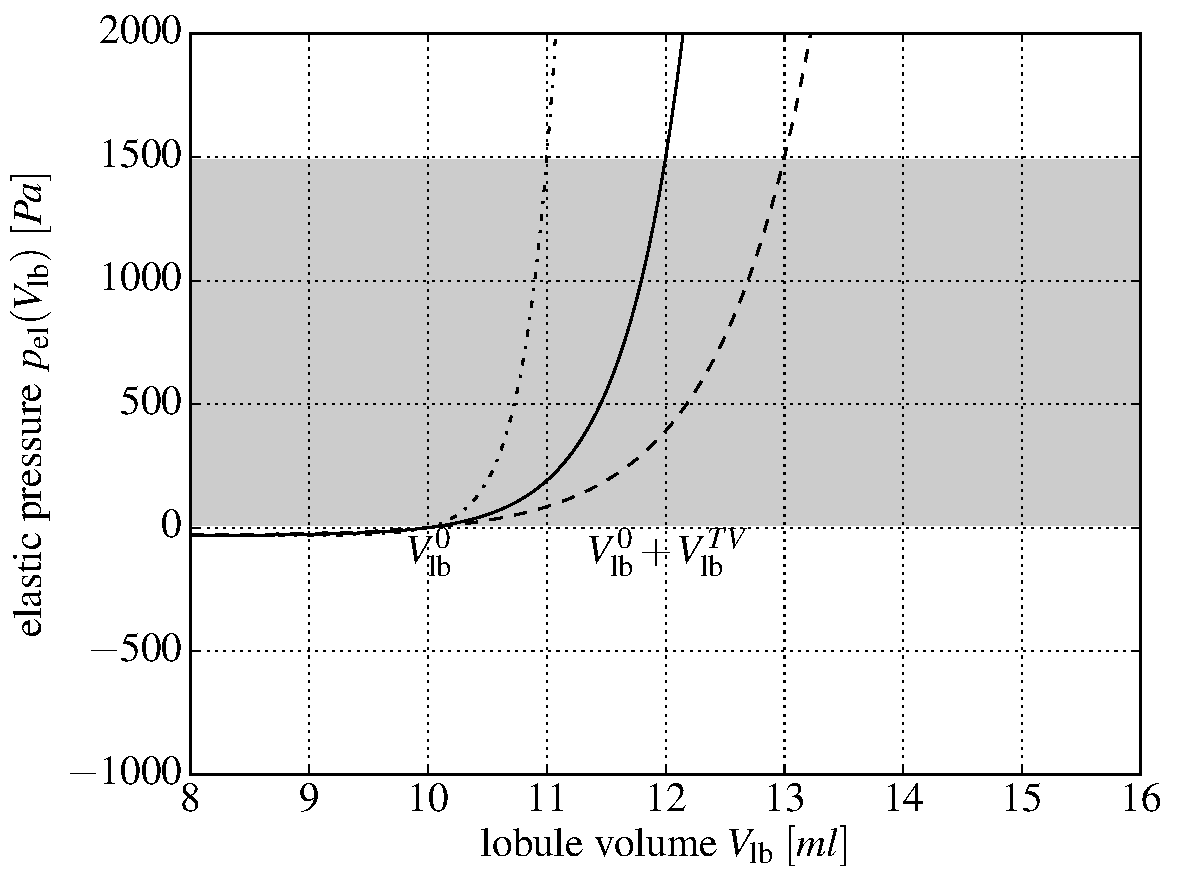
\includegraphics[width=0.5\textwidth]{figures/lobule_mechanics}
  \caption{Elastic pressure for a stiff (dash-dotted line), medium (solid line) and soft (dashed line) trumpet-lobule. Grey zone indicates range of transacinar pressure resulting from typical pleural pressure.}
  \label{fig:lobuleMechanics}
\end{figure}


\subsection{Distribution of the modification parameters}
In the analysis of structural inhomogeneities it can be distinguished between global, regional, and local differences in the lung structure, i.e. in the modification parameters acting on the mechanical and geometrical properties of the lung model.
In the case of global type inhomogeneities, the lung modification parameters ($\phi$, $\theta$, $\tau$) are specified for all trumpet modules in the entire model.
Thereby, the parameters are sampled either from a log-normal distribution (global I), where the variability is set based on the mean and the standard deviation ($\sigma$) of the normal distribution of the parameter, or from a linear function returning increasing values from one element to the next within a specified range $\hat\sigma$ (global II).
For regional type inhomogeneities, lung modification parameters are set to specific values for a certain fraction of all trumpet lobules.
Thereby, all affected units lie in the same region, although they do not necessarily share a common bronchiole, with respect to the morphology of the model lung.
Local type inhomogeneities are defined in a similar way as regional type inhomogeneities with the difference that the subsets of modified units are distributed uniformly across the lung model.


%********************* NEW SECTION *********************
%-------------------------------------------------------
\section{Numerical implementation} \label{sec:numerical_implementation}
Lorem ipsum dolor sit amet, consetetur sadipscing elitr, sed diam nonumy eirmod tempor invidunt ut labore et dolore magna aliquyam erat, sed diam voluptua. At vero eos et accusam et justo duo dolores et ea rebum. Stet clita kasd gubergren, no sea takimata sanctus est Lorem ipsum dolor sit amet. Lorem ipsum dolor sit amet, consetetur sadipscing elitr, sed diam nonumy eirmod tempor invidunt ut labore et dolore magna aliquyam erat, sed diam voluptua.


%****************** new sub-section ********************
\subsection{Ventilaton lumped parameter model} \label{ssec:ventilation}
\subsubsection{Duct-like airways}
Regarding airflow in duct-like airways, we applied Womersley's theory for pulsatile flow in tubes \cite{Womersley1957}.
For this case, the pressure difference between two subsequent nodes with index $i$ and $j$ in the network reads,
\begin{equation}
p_i - p_j = R_{ij} Q_{ij}\cc \quad{\mathrm{with}}\quad R_{ij} = \Re\left\{\frac{\i \omega \rho l_{ij}}{r_{ij}^2 \pi}\left[1-\frac{2\mathsf{J_1}(\i^{3/2}\alpha)}{\i^{3/2}\alpha \mathsf{J_2}(\i^{3/2}\alpha)}\right]^{-1}\right\} \pp
\end{equation}
Here, $R_{ij}$ is the hydrodynamic resistance and $Q_{ij}$ the flow rate in the conducting airway between nodes $i$ and $j$; $\alpha = r_{ij}\sqrt{\omega\rho/\mu}$ is known as the Womersley number, $\omega = 2\pi/T_\mathrm{B}$ is the breathing frequency related to the breath period $T_\mathrm{B}$; $r_{ij}$ and $l_{ij}$ are the radius and the length, respectivel, of the conducting airway; $\mu$ is the dynamic viscosity, and $\rho$ the density of air; and $\i = \sqrt{-1}$.

To save computation time in the simulations, the resistance $R_{ij}$ is interpolated from a previously computed table for different diameters and breath periods.

\subsubsection{Compliant trumpet lobules}
For the constitutive law of the trumpet lobules, we used used an exponential relation between the elastic pressure and the (tidal) volume of the lobule.
Additionally a pressure loss was introduced due to the hydrodynamic flow resistance in the lobule.
Referring to Figure \ref{fig:network} for notations, the total pressure drop of a trumpet lobule can be stated as

\begin{figure}[b!]
\centering
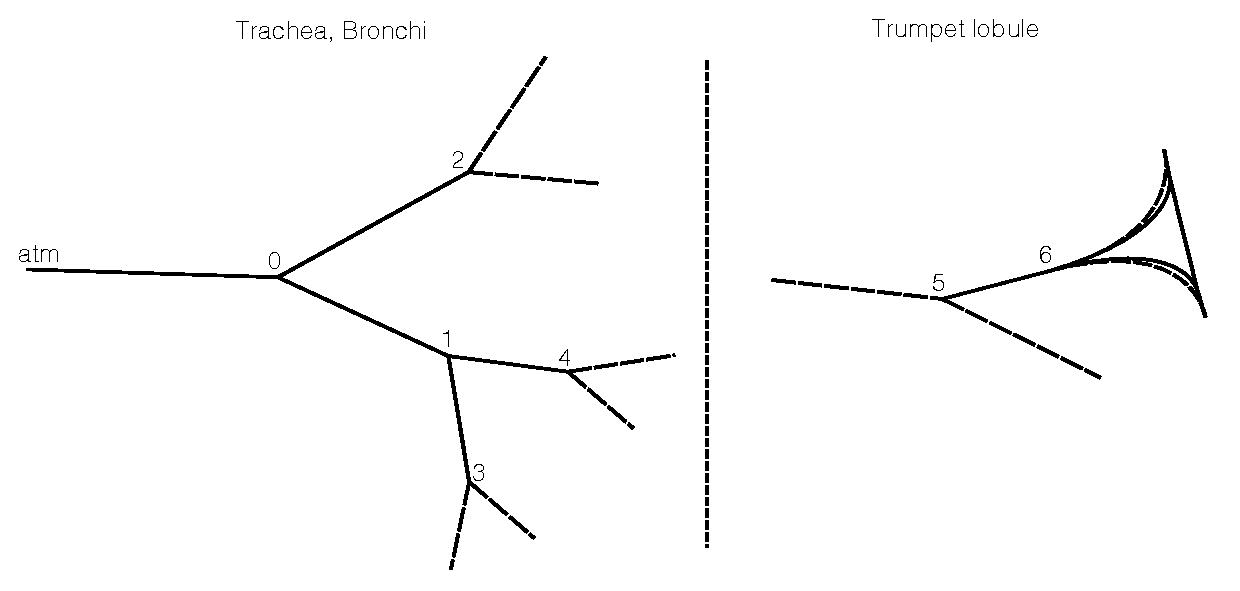
\includegraphics[width=\textwidth]{figures/network}
\caption{Reduced size network of duct-like airways and trumpet lobule at the periphery}
\label{fig:network}
\end{figure}

\begin{equation} \label{eqn:governingequation}
p_6 - p_\pl = R_\lb Q_\ter + \beta\e^{\gamma V_\lb^0}\left(\e^{\gamma \tilde{V}_\lb} - 1 \right) \cc
\end{equation}

where $p_6$ is the pressure at the end of a duct-like airway feeding into a trumpet-lobule, $p_\pl$ is the pressure in the pleural cap, $R_\lb$ is the total hydrodynamic resistance within the trumpet lobule, $Q_\ter = \d V_\lb / \d t$ is the flow rate at the inlet of the lobule, and $V_\lb$ is the lobule volume.
The parameters $\beta$ and $\gamma$ were determined by the choice of a specific material law with its characteristic compliance and non-linearity (Equ. 3 in the main article).
The lobule volume can be decomposed into a static part, $V_\lb^0$ determined by the number of trumpet lobules and the functional residual capacity (FRC), and a dynamic part which varies during tidal breathing

\begin{equation}
V_\lb = V_\lb^0 + \tilde{V}_\lb \pp
\end{equation}

Differentiation of equation (\ref{eqn:governingequation}) with respect to time and rearranging yields

\begin{equation} \label{eqn:differentialEquationI}
\frac{\d Q_\ter}{\d t} = \frac{1}{R_\lb}\left[ -\gamma\beta\e^{\gamma V_\lb}Q_\ter + \left(\frac{\d p_6}{\d t} - \frac{\d p_\pl}{\d t}\right)\right] \pp
\end{equation}

Replacing the flow rate in the terminal duct with $Q_\ter = T_{56}(p_5 - p_6)$, with $T_{56}$ the transmissibility (inverse of resistance) in the terminal conducting airway between nodes $5$ and $6$, the differential equation (\ref{eqn:differentialEquationI}) can be written in the form

\begin{equation} \label{eqn:differentialEquationII}
  \frac{\d p_6}{\d t} - \frac{\d p_\pl}{\d t} - R_\lb T_{56}\left(\frac{\d p_5}{\d t} - \frac{\d p_6}{\d t}\right) = T_{56}\gamma\beta\e^{\gamma V_\lb}\left( p_5 - p_6\right)
\end{equation}


\subsubsection{Numerical solution}
We applied the trapezoidal rule for the numerical integration of Equation (\ref{eqn:differentialEquationII}).

\begin{equation}
\begin{split} \label{eqn:discreteODEI}
(p_6^n - p_6^{n-1}) - (p_\pl^n - p_\pl^{n-1}) - R_\lb T_{56} \left[ (p_5^n - p_5^{n-1}) - (p_6^n - p_6^{n-1})\right] \\
= \frac{\Delta t}{2}T_{56}\gamma\beta\e^{\gamma V_\lb^\star}\left[ (p_5^n + p_5^{n-1}) - (p_6^n + p_6^{n-1})\right]
\end{split}
\end{equation}

Here, $(.)^n$ denotes variables at the new, updated, discrete time $t = n\Delta t$, with $\Delta t$ the time step.
The lobular volume at timestep $n$ is estimated using an explicite Euler formulation $V_\lb^\star = V_\lb^{n-1} + \Delta t Q_\ter^{n-1}$.
For implementation purposes, Equation (\ref{eqn:discreteODEI}) is reformulated as

\begin{equation} \label{eqn:discreteODEII}
  -K_1 p_5^n + (1 + K_1) p_6^n - p_\pl^n = K_2
\end{equation}

where the two coefficients $K_1$ and $K_2$ are computed based on available information from the former time step.

\begin{align}
  K_1 &= R_\lb T_{56} + \frac{\Delta t}{2}T_{56}\gamma\beta\e^{\gamma V_\lb^\star} \\
  K_2 &= -R_\lb T_{56} p_5^{n-1} + \left( 1 + R_\lb T_{56}\right) p_6^{n-1} - p_\pl^{n-1} + \frac{\Delta t}{2}T_{56}\gamma\beta\e^{\gamma V_\lb^\star}\left( p_5^{n-1} - p_6^{n-1}\right)
\end{align}

At bifurcations of duct-like airways, the flow balance has to be satisfied in each time step.
Referring to node $1$ in Figure \ref{fig:network} this reads

\begin{equation} \label{eqn:flowBalance}
\begin{split}
Q_{01}^n - Q_{13}^n - Q_{14}^n &= 0 \\
T_{01}(p_0^n - p_1^n) - T_{13}(p_1^n - p_3^n) - T_{14}(p_1^n - p_4^n) &= 0
\end{split}
\end{equation}

subject to boundary conditions imposed at the inlet of the airway tree,

\begin{equation}
T_\mathrm{tr}(p_\mathrm{atm} - p_0) = Q_\mathrm{in}(t)
\end{equation}

The flow rate profile $Q_\mathrm{in}(t)$ was pre-defined and constant atmospheric pressure was assumed at the inlet.
$T_\mathrm{tr}$ is the transmissibility of the trachea and $p_0$ the pressure in the first bifurcation.
Equations (\ref{eqn:discreteODEII}) and (\ref{eqn:flowBalance}) can be stated for all bifurcation nodes and lobules.
Together with the boundary conditions this yields a system of equations for the pressure values in the bifurcation nodes, $p_i$, and the pleural pressure, $p_\pl$, which had to be solved in each time step.
Thereby, for each discrete time-step, a uniform pleural pressure was assumed.
To solve the resulting system of equations, we applied an iterative method (bi conjugate gradient stabilized solver) from the EIGEN linear algebra library (eigen.tuxfamily.org).


%****************** new sub-section ********************
\subsection{Gas transport equation} \label{ssec:gas}
For the transport of an inert gas in the lung two transport mechanism were considered: Advection (in this context also called convection) and molecular diffusion.
More information about the underlying assumptions are given in the method section of the main article.
The 1D-advection-diffusion equation governs the evolution of the gas concentration $c = c(x,t)$ (normalized with the maximum concentration, $c\in[0,1]$) in time and along the airway streamwise coordinate $x$:

\begin{equation} \label{eqn:advection_diffusion}
\frac{\partial c}{\partial t} = -\underbrace{u\frac{\partial c}{\partial x}}_{\text{\footnotesize{advection}}} + \underbrace{D\frac{\partial^2 c}{\partial x^2}}_{\text{\footnotesize{diffusion}}}
\end{equation}

In the lung model the velocity $u$ was computed by means of a lumped parameter (0D) model for the ventilation of all model airway (see S1\_Appendix), and the diffusion coefficient $D$, given the properties of both the carrier gas and the inert tracer gas, was computed using Chapman-Enskog equation.
In addition, $D$ was modified to account for Taylor's dispersion (see \cite{Cussler2009}).
For the discretization of Equation (\ref{eqn:advection_diffusion}) the advection velocity $u$ was assumed to be constant within a duct-like airway.
Transport phenomena related to spacial velocity gradients at the bifurcations are not considered.
In trumpet lobules, the non-constant cross-section lead to a modified advection velocity $\hat u$ (see Appendix\_S01).
Otherwise the numerical treatment was the same for duct-like airways and trumpet lobules.
A duct or trumpet lobule was discretized into $N$ elements and hence Equation (\ref{eqn:advection_diffusion}) is evaluated on $N+1$ nodes, where $N$ can be different for each airway.
The avection-diffuison equation (\ref{eqn:advection_diffusion}) was discretized applying a second order upwind scheme and a second order central scheme for the spatial discretization of the advection term and the diffusion term, respectively, and using a generalized Crank-Nicolsen scheme for the temporal discretization.

\begin{equation} \label{eqn:advection_diffusion_discr1}
\frac{\underline{c}^{n+1} - \underline{c}^{n}}{\Delta t} = \theta(-u\underline{\underline{\mathcal{D}_1}} + D \underline{\underline{\mathcal{D}_2}})\underline{c}^{n+1} + (1 - \theta)(-u\underline{\underline{\mathcal{D}_1}} + D \underline{\underline{\mathcal{D}_2}})\underline{c}^{n} + \underline{b}^n
\end{equation}

Here, $\underline{c}$ is the vector containing the $N+1$ concentration values within the given airway model, $\underline{\underline{\mathcal{D}_1}}$ and $\underline{\underline{\mathcal{D}_2}}$ are finite difference operators for the first, respectively the second spatial derivatives, and $\underline{b}$ are boundary conditions containing information from the neighboring ducts.
The superscript $n$ refers to the time step $t_n = n \Delta t$.
Equation (\ref{eqn:advection_diffusion_discr1}) is partly implicite due to the concentration vector considered at the new (updated) time step  $t_{n+1}$ appearing on the right-hand side.
The coefficient $\theta \in [0, 1]$ controls the weight of the implicite information (at $t_{n+1}$).
For all simulations $\theta = 0.7$ was used.
Rearranging the discretized advection-diffusion equation yields a linear system for the concentration values at the new time-step $\underline{c}^{n+1}$.

\begin{equation} \label{eqn:advection_diffusion_discr2}
\underbrace{\left[1 - \Delta t \theta(-u\underline{\underline{\mathcal{D}_1}} + D \underline{\underline{\mathcal{D}_2}})) \right]}_{=:\underline{\underline{\mathcal{L}}}} \underline{c}^{n+1} = \underbrace{\left[1 + \Delta t(1-\theta)(-u\underline{\underline{\mathcal{D}_1}} + D \underline{\underline{\mathcal{D}_2}})) \right]}_{=:\underline{\underline{\mathcal{R}}}} \underline{c}^{n}  + \Delta t\underline{b}^n
\end{equation}

Considering the gridsize $h$ of the 1D mesh in a duct or trumpet-like structure, the upwind operator $\underline{\underline{\mathcal{D}_1}}$ was chosen according to the flow direction during inspiration and expiration:

\begin{equation}
\begin{split}
\text{if }u \geq 0 \text{:}&\quad
\underline{\underline{\mathcal{D}_1}} = \frac{1}{2h}
\left[\begin{array}{ccccccc} 3 &  0 &  \dots & \dots & \dots & \dots & 0 \\
                            -4 &  3 &  0 & \dots & \dots & \dots & \vdots  \\
                             1 & -4 &  3 & 0 & \dots & \dots & \vdots \\
                             0 &  1 & -4 &  3  & 0 & \dots & \vdots \\
                             \vdots  & \ddots & \ddots & \ddots  &\ddots & \ddots & \vdots \\
                             \vdots  & \dots & 0 & 1 & -4 & 3 & 0 \\
                             0 & \dots & \dots & 0 & 1 & -4 & 3 \\\end{array}\right] \\ \\
\text{if }u < 0 \text{:}&\quad
\underline{\underline{\mathcal{D}_1}} = \frac{1}{2h}
\left[\begin{array}{ccccccc} -3 &  4 &  -1 & 0 & \dots & \dots & 0 \\
                              0 & -3 & 4 & -1 & 0 & \dots & \vdots  \\
                              \vdots & \ddots & \ddots & \ddots & \ddots & \ddots & \vdots \\
                              \vdots &  \dots & 0 & -3 & 4 & -1 & 0 \\
                              \vdots  & \dots & \dots & 0 & -3 & 4 & -1 \\
                              \vdots  & \dots & \dots & \dots & 0 & -3 & 4 \\
                              0 & \dots & \dots & \dots & \dots & 0 & -3 \\\end{array}\right]
\end{split}
\end{equation}

The finite difference operator for the second spatial derivative is given by

\begin{equation}
\underline{\underline{\mathcal{D}_2}} = \frac{1}{h^2}
\left[\begin{array}{ccccccc} -2 &  1 &  0 & \dots & \dots & \dots & 0 \\
                              1 & -2 & 1 & 0 & \dots & \dots & \vdots  \\
                              0 &  1 & -2 & 1 & 0 & \dots & \vdots  \\
                              \vdots & \ddots & \ddots & \ddots & \ddots & \ddots & \vdots \\
                              \vdots  & \dots & 0 & 1 & -2 & 1 & 0 \\
                              \vdots & \dots & \dots & 0 & 1 & -2 & 1 \\
                              0 & \dots & \dots & \dots & 0 & 1 & -2 \\\end{array}\right]
\end{equation}

\subsubsection{Boundary conditions}
\paragraph{Bifurcation boundary conditions:}

\begin{figure}[b!]
\centering
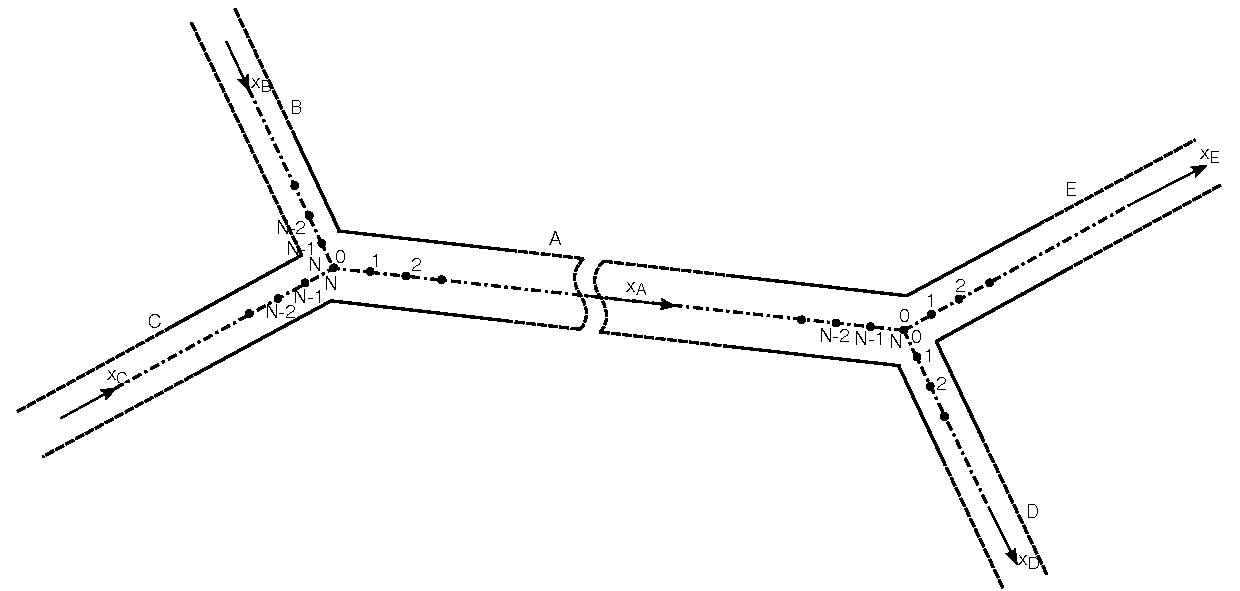
\includegraphics[width=\textwidth]{figures/bifurcation_nodecentered}
\caption{Bifurcation of duct-like airways with one-dimensional grid for gas transport.}
\label{fig:bifurcation}
\end{figure}

Referring to the schematic in Figure \ref{fig:bifurcation}, boundary conditions for the airway A can be stated based on the concentrations in the last nodes of airways $B$ \& $C$ or of the first nodes in airways $D$ \& $E$, depending on the advection direction.
The contributions of each airway $B$ \& $C$ or $D$ \& $E$ were weighted by the specific flow rates or cross-sections in the corresponding neighboring airways.
In the following, we state the bifurcation boundary conditions for $A$ for positive flow ($u_A>0$), where airways $B$ \& $C$ feed into airway $A$, which feeds into airways $D$ \& $E$, and for negative flow ($u_A<0$), where airways $D$ \& $E$ feed into airway $A$, which feeds into airways $B$ \& $C$.
The bifurcation boundary conditions were implemented by means of ghost-nodes up-stream and down-stream of a given airway.
For the considered case the ghost cell concentration values read

\begin{equation}
\begin{split}
c_{A_{-1}}^\mathrm{adv}  &= \frac{|Q_B|}{|Q_B| + |Q_C|}c_{B_{N}}^\star + \frac{|Q_C|}{|Q_B| + |Q_C|}c_{C_{N}}^\star \\
c_{A_{-2}}^\mathrm{adv}  &= \frac{|Q_B|}{|Q_B| + |Q_C|}c_{B_{N-1}}^\star + \frac{|Q_C|}{|Q_B| + |Q_C|}c_{C_{N-1}}^\star \\
c_{A_{N+1}}^\mathrm{adv} &= \frac{|Q_D|}{|Q_D| + |Q_E|}c_{D_{1}}^\star + \frac{|Q_E|}{|Q_D| + |Q_E|}c_{E_{1}}^\star \\
c_{A_{N+2}}^\mathrm{adv} &= \frac{|Q_D|}{|Q_D| + |Q_E|}c_{D_{2}}^\star + \frac{|Q_E|}{|Q_D| + |Q_E|}c_{E_{2}}^\star \\
\\
c_{A_{-1}}^\mathrm{dif}  &= \frac{|S_B|}{|S_B| + |S_C|}c_{B_{N}}^\star + \frac{|S_C|}{|S_B| + |S_C|}c_{C_{N}}^\star \\
c_{A_{N+1}}^\mathrm{dif} &= \frac{|S_D|}{|S_D| + |S_E|}c_{D_{1}}^\star + \frac{|S_E|}{|S_D| + |S_E|}c_{E_{1}}^\star \\
\end{split}
\end{equation}

where $Q_B, Q_C, Q_D, Q_E$ are the flow rates in the neighboring airways of $A$, and $c^\star$ denotes a concentration value in neighboring duct interpolated onto a grid with the same grid-size as the considered airway $A$.
Using these values, the bifurcation boundary conditions in equation (\ref{eqn:advection_diffusion_discr2}) were introduced with the vector $\underline{b}$ as follows

\begin{equation}
\begin{split}
\text{if }u \geq 0 \text{:}&\quad
\underline{b} =
\left(\begin{array}{c} \frac{-u_A}{2h}\left( -4 c_{A_{-1}}^\mathrm{adv} + c_{A_{-2}}^\mathrm{adv}\right) + \frac{D}{h^2}c_{A_{-1}}^\mathrm{dif} \\
                       \frac{-u_A}{2h}c_{A_{-2}}^\mathrm{adv} \\
                       0 \\
                       \vdots \\
                       + \frac{D}{h^2}c_{A_{N+1}}^\mathrm{dif} \end{array}\right) \\ \\
\text{if }u < 0 \text{:}&\quad
\underline{b} =
\left(\begin{array}{c} \frac{D}{h^2}c_{A_{-1}}^\mathrm{dif} \\
                       \vdots \\
                       0 \\
                       \frac{-u_A}{2h}(-c_{A_{N+1}}) \\
                       \frac{-u_A}{2h}\left(4 c_{A_{N+1}} - c_{A_{N+2}}\right) + \frac{D}{h^2}c_{A_{N+1}} \end{array}\right)
\end{split}
\end{equation}

\paragraph{Inlet boundary conditions:}
At the inlet (mouth), boundary conditions of Dirichlet type, $c_0 = 1$, for inspiration, and Neumann type, $-4c_0 + 3c_1 -1c_2 = 0$, for expiration were chosen.
The left and right-hand operator, $\mathcal{L}$ and $\mathcal{R}$ respectively, in Equation (\ref{eqn:advection_diffusion_discr2}) were modified accordingly.

\subsection*{Time-step and grid size}
The time-step size $\Delta$ was linked to the grid-size $h$ by means of the well known CFL condition.
\begin{equation}
  h = \frac{u \Delta t}{CFL}
\end{equation}
Considering a given time step $\Delta t$, the number of elements of a 1D mesh of length $l = N h$ (in either duct-like airways or a trumpet module) was fixed as
\begin{equation}
  N = \texttt{floor}\left\{\frac{l\;CFL}{u \Delta t}\right\}
\end{equation}
where $CFL=1.0$ was used for all simulations.

If faster advection velocities (e.g. during peak inspiration or expiration) causes the number of elements to drop bellow a defined minimal number
$N_\mathrm{min}$, a time-step refinement $\Delta t / n_\mathrm{tsr}$ was activated, which was computed as
\begin{equation}
  n_\mathrm{tsr} = \frac{u \Delta t N_\mathrm{min}}{l\;CFL}
\end{equation}
The refined time-step $\Delta t / n_\mathrm{tsr}$ was then used for the numerical solution.



%********************* NEW SECTION *********************
%-------------------------------------------------------
\section{Code structure} \label{sec:code_structure}
The computer code is implemented in C++.
The computer code consists of four objects (classes) (\texttt{lung.cpp}, \texttt{duct.cpp}, \texttt{lobule.cpp}, \texttt{gas.cpp}) which constitute the lung model.
The remaining source files relate to the procedural aspects of the simulation and data handling.
An overview of the whole environment of the model is explained in more detail in Section \ref{sec:environment} in the upcoming chapter.
Here, the main procedural structure of the solver, wich are defined in \texttt{main.cpp} and \texttt{flDriver.cpp}, are outlined, and the architecture of the lung model is shown schematically.

\subsubsection{Input / Output}
Reading and writing of input, respectively output data is defined in \texttt{main.cpp}, which also contains the simulation start command via the
call of a driver.
The structure is as follows:
\begin{itemize}
  \item Reading system (model) parameters and simulation control parameters from input files.
  \item Dynamically allocate and stock containers for these parameteres.
  \item Dynamically allocate (no stocking yet) containers for simulation outputs / results.
  \item Call of driver for simulation.
  \item Write output containters to local environment.
\end{itemize}

\subsubsection{Model built \& simulation}
The driver \texttt{flDriver.cpp} called in \texttt{main.cpp} first builds the model accoring to a parametrized fractal morphology and initializes its member variables.
After this the simulation time loop is started in which the different (per-time-step) numerical commands are called.
The structure is as follows:
\begin{itemize}
  \item Construct lung object (see model architecture bellow).
  \item Generate fractal tree of duct-like airways.
  \item Generate / Add trumpet-lobules at the end of each terminal duct.
  \item Pass input data (e.g. flow rate profile, breath periode) to lung model.
  \item Read and apply lung modification instructions (e.g. for lobular compliance modification $\phi$)
  \item Allocate / Initialize vectors and matrices for ventilation LPM (linear system).
  \item Define gridsize.
  \item Setup gas object.
  \item Start time loop:
  \begin{itemize}
    \item Reset breath period if necessary.
    \item Compute time step refinement (TSR).
    \item Start inner loop (according to TSR):
    \begin{itemize}
      \item Write entries in system matrix and right-hand side vector for ventilation LPM.
      \item Solve for pressure and distribute to nodes in LPM.
      \item Compue flow rate in each duct-like airway.
      \item Update trumpet-lobule dynamics.
      \item Update concentration in 1D domains (domain decomposition approach).
    \end{itemize}
    \item Write results of current time step to output data containers.
  \end{itemize}
\end{itemize}


\subsubsection{Model architecture}
The numerical model of the lung consits of four different objects: The lung-object (\texttt{lung.cpp}) governs the construction of the model and the all calls of numerical computations within the different lung units (i.e. ducts and lobules).
Computations or data passing that are applied to all (or certain) lung units, a recursive implementation is chosen.
E.g. the rules to grow (or stop growing) daughter ducts according to Equation (\ref{eqn:bifurcationRule}) are the same for all ducts.
Therefore it is handy to implement only the rule and then apply it via recursion to all ducts and lobules withing the tree-like morphology
This concept is applied for many operational steps of the model.
The strict implementation of recursion for this type of domain morphology also assures that the domains are scaned / traveled in a predefined manner, which eases the right allocations of different units or nodes.
The lung-object points (via pointer \textit{pTrachea}) on a fractal tree of duct-objets (\texttt{duct.cpp}).
A duct-like airways is connected (via pointers \textit{pParent}, \textit{pMinoDaughter}, \textit{pMajorDaughter}) to the neighoring branches (ducts).
Terminal ducts (defined by $d_\mathrm{Lim}$) are connected to a lobule-object (\texttt{lobule.cpp}, via pointer \textit{pMinoDaughter})
Each duct and lobule is associated with a proper gas object.
A Schematics of this architecture is shown in Figure ...
